% doc class article- for research papers
\documentclass[fleqn]{article}

% installing necessary packages
\usepackage[english]{babel}
\usepackage{amssymb}
\usepackage[a4paper,top=2cm,bottom=2cm,left=3cm,right=2cm,marginparwidth=1.75cm]{geometry}
\usepackage{amsmath}
\usepackage{graphicx}
\usepackage[colorlinks=true, allcolors=blue]{hyperref}
\usepackage{bookmark}
\usepackage{tikz}
\usetikzlibrary{calc}

% command for inserting keyowrds after the abstract
\providecommand{\keywords}[1]
{
  \small	
  \textbf{\textit{Keywords---}} #1
}

% command for inserting border on the title page
\newcommand\HRule{\rule{\textwidth}{1pt}}

% begin the main content of the document
\begin{document}

% all the description of the very frist title page
\begin{titlepage}
\begin{tikzpicture}[remember picture, overlay]
    \draw[line width = 1pt] ($(current page.north west) + (0.7in,-1in)$) rectangle ($(current page.south east) + (-0.7in,1in)$);
\end{tikzpicture}

\begin{center}
    \vspace*{2cm}    
    \Large
    \textbf{Why High-Order Polynomials Should Not be Used in
    Regression Discontinuity Designs -A Review}
        
    \vspace{3.5cm}
    \large
    Research Paper Presented to the \\
    \vspace{0.2cm}
    Department of Economics at the\\
    \vspace{0.2cm}
    Rheinische Friedrich-Wilhelms-Universität Bonn
        
    \vspace{1.5cm}

    In Partial Fulfillment of the Requirements for the Degree of\\ 
    \vspace{0.2cm}
    Master of Science (M.Sc.)
    
    \vspace{2cm}    
    \includegraphics[width=0.2\textwidth]{uni-bon-logo.png}

    \vspace{2.5cm}
    \large
    Submitted to: Prof. Dr. Christoph Breunig and Dr. Dennis Schroers\\
    \vspace{2cm}
    Submitted in February 2023 by:\\
    \vspace{0.2cm}
    Raunak Mehrotra and Vanshaj Bindlish\\
    \vspace{0.2cm}
    Matriculation Number: 3391327 and 3466315
\end{center}
\end{titlepage}

\vspace*{2cm}
\tableofcontents
\hypersetup{hypertexnames=false}
\newpage

\begin{abstract}
     Controlling for higher degrees of polynomials for the forcing variable is a common practice in regression discontinuity analysis. Such models can overfit, resulting in substantively implausible causal inferences that randomly contribute variation to the high-degree polynomial and can lead to false estimates. The aim of this paper is to investigate the three arguments presented in Gelman and Imbens (2019)\cite{gelman2019high}. The arguments recommends against the use of high-order polynomial approximations are: the implicit weights are inappropriate, the estimates are sensitive to the degree of polynomial, and poor coverage of confidence intervals. Instead, the paper suggests using local linear or quadratic polynomial approximations.
\end{abstract}\hspace{10pt}

\keywords {Causal inference, Treatment effect, Regression discontinuity, Polynomial Regression.}

\section{Introduction}
\phantomsection\label{sec:intro}


    Regression discontinuity designs have significantly gained importance in econometric and causal inference over the past few decades. Introduced in 1960 by Donald L. Thistlethwaite and Donald T. Campbell \cite{thistlethwaite1960regression}, the regression discontinuity design aims to estimate the impact of a treatment policy on the variable of interest. The simplicity of the design enables its application across research fields, like health, labor, education, political economy, etc. \\

    The basic idea behind the regression discontinuity (RD) design is that the allotment of the treatment is based on the value of the predictor (also known as assignment/forcing variable) being on either side of a fixed threshold \cite{imbens2008regression}. Further, the assignment variable may be related to the potential outcome, however, this relation is assumed to be smooth\footnote{that is, all other factors determining Y must be evolving smoothly with respect to X} which implies that any discontinuity at the cutoff point in the conditional expectation of the outcome as a function of the assignment variable is because of the treatment and this discontinuity gap represents the causal effect of the treatment. For instance, Thistlethwaite and Campbell \cite{thistlethwaite1960regression} studied the role of merit awards on future academic outcomes by allocating awards only to the students who had scored above a threshold score value in a test, while the students who scored below the cutoff point did not receive any award. \\

    The aforementioned RD design is known as Sharp Regression Discontinuity (SRD) which is hereby used for all purposes of the study and used interchangeably with regression discontinuity (RD) in the paper. From the above design, we can infer that for each individual $i$ there exists a pair of potential outcomes: $Y_{i}(0)$ and $Y_{i}(1)$, where the latter denotes the outcome if an individual $i$ has been assigned the treatment and the former denotes the outcome if the treatment has not been assigned. In causal inference, we are interested in $Y_{i}(1) - Y_{i}(0)$, that is, the treatment effect. However, since the outcomes $Y_{i}(0)$ and $Y_{i}(1)$ for an individual $i$ cannot be observed at the same time, it is typically the average of the treatment effect ($Y_{i}(1)$) which is calculated over the (sub-)populations\cite{imbens2008regression}. \\

    In an RD setting, then for an assignment variable $X$ with the threshold point at $c$, $\mathbb{E} [ Y_{i}(1) | X ]$ and $\mathbb{E} [ Y_{i}(0) | X ]$ represent the average outcome conditional on the assignment variable if an individual $i$ has been assigned the treatment or not, respectively. But as only those individuals in $X$ with a value above the threshold are assigned the treatment, we only observe $\mathbb{E} [ Y_{i}(1) | X ]$ to the right of the threshold and $\mathbb{E} [ Y_{i}(0) | X ]$ to the left of the threshold. Therefore, the earlier mentioned continuity assumption enables us to use the average outcome of those who didn't receive the treatment as a valid counterfactual for those who received the treatment and hence, calculate the average treatment effect(ATE)\cite{lee2010regression}.\\

    Based on the above specification, the average treatment effect can be estimated as the discontinuity in the conditional expectation of the outcome given the assignment variable at the threshold: \\
    \begin{equation*}
        \qquad \tau_{SRD} = \lim_{x\downarrow c} \mathbb{E}[Y_{i} | X_{i}=x] - \lim_{x\uparrow c} \mathbb{E}\left[Y_{i} | X_{i}=x\right]    
    \end{equation*}

    which is equal to \\
    \begin{equation*}
        \qquad \tau_{SRD} = \mathbb{E}\left[Y_{i}(1) - Y_{i}(0)| X = c\right]    
    \end{equation*}

    Here, $\tau_{SRD}$ is the 'Average Treatment Effect' at threshold $c$.\\

    This can also be seen in Figure \ref{fig:sharp_rdd}, which illustrates a sharp RD design with the threshold at $6$. Individuals right to the threshold are given the treatment, while those to the left are the control group. The dashed line represents the value of the potential outcome for the treated group and control group if they were observable beyond their treatment status. The smooth lines indicate the observed outcome conditional on the assignment variable. Under the continuity assumption, therefore, the average treatment effect, $\tau_{SRD}$ is given by the jump in outcome value at threshold $6$.  \\

    \begin{figure}[h]
        \centering
        \includegraphics[width = 15cm,height = 5cm]{Intro Sharp RDD.png}
        \caption{Sharp RDD*}
        \small\textsuperscript{*}Sourced from Imbens and Lemieux (2007)\cite{imbens2008regression}. X-Axis is the forcing variable, while Y-Axis is the outcome value 
        \label{fig:sharp_rdd}
    \end{figure}

    The next challenge now is to estimate: \\
    \begin{equation*}
        \qquad \mu_{+} = \lim_{x\downarrow c} \mathbb{E}\left[Y_{i} | X_{i}=x\right] \\and,
        \qquad \mu_{-} = \lim_{x\uparrow c} \mathbb{E}\left[Y_{i} | X_{i}=x\right]
    \end{equation*}

    Since researchers are often unsure about the efficiency of the estimates based on global linear function\cite{gelman2019high}, they often use polynomial functions of order fifth or sixth of the assignment variable, $X$ in the regression model. The appropriate degree of polynomial is mainly selected based on some statistical information criteria (like goodness-of-fit) or cross-validation.\\
    
    The other approach to estimate $\mu_{+}$ and $\mu_{-}$ and consequently the treatment effect is to use local low-order (linear or quadratic) polynomial approximation. In this method, the values of $x_{i}$ around the threshold $c$ that lie within the bandwidth $h$ are used to estimate a linear or quadratic function, while the rest of the values of $x_{i}$ are discarded. Several methods have been developed to estimate the value of h (see Imbens and Kalyanaraman(2012)\cite{imbens2012optimal}, Hahn, Todd, and Van Der Klaauw (2001)\cite{hahn2001identification}, Lee and Lemieux(2010) \cite{lee2010regression}).\\

    Gelman and Imbens(2019)\cite{gelman2019high} believe that the former approach, that is, to use the global high-order polynomials to estimate the causal treatment effect is flawed and rather the inference should be based on local low-order polynomials. The authors bring forth threefold arguments to show global high-order polynomials as a poor model choice for regression discontinuity analysis.\\

    \begin{itemize}
        \item The first argument is that the estimates of the treatment effect can be driven by the values of the forcing variable that are away from the threshold. Since the RD estimate is the difference between the weighted average of the outcome for the treated and untreated, wherein the weights depend only on the forcing variable; the weights in a global high-order polynomial approximation are extreme and unattractive compared to a local linear/quadratic approximation.
        \item The second argument put forward is that the estimates in the case of global high-order polynomials are highly sensitive to the chosen degree of the polynomial of the forcing variable $X$. Further, a lack of just criteria to select the order of polynomials that is suitable for the estimator to satisfy its objectives of causal inference exacerbates the issue.
        \item Finally, the third argument is that the confidence interval based on the estimates of global high-order polynomials is often misleading. The confidence intervals can be too narrow that they reject the null hypothesis even when it shouldn't have, that is, the probability of Type 1 error rate is much higher than the nominal rate of 5\%. This implies that there is a higher bias in the case of global high-order polynomials to detect a discontinuity even if there isn't one, and hence, generate poor inference.
    \end{itemize}

    The target of our paper is to test the veracity of these arguments through a simulation study and empirical application (wherever possible). The paper hereby proceeds as follows. In the next section, we introduce the model specification of the RD design that is used to critique the aforementioned arguments. Thereafter, we evaluate our results based on the simulation and empirical evidence so as to comment on the feasibility of global high-order polynomials in RD design.\\

    \section{Methodology}
    \phantomsection\label{sec:methodology}
    
    \subsection{General Framework}
    \phantomsection\label{subsuc:general framework}
    
    In practice, it is convenient to run a pooled regression to obtain the average treatment effect of the SRD rather than to estimate the values of $\mu_{+}$ and $\mu_{-}$ and then take their difference. This general approach of pooled regression based on Lee and Lemieux (2010)\cite{lee2010regression} can be represented as:\\
    \begin{equation*}
        \qquad Y = \beta_{1} + \tau_{SRD} D + f(X-c) + \epsilon
    \end{equation*}

    Where, $\beta_{1}$ is the intercept term and equal to ($\beta_{1}^{+} - \beta_{1}^{-}$)\footnote{Here and in the consequent equations of Sec 2.1, the superscript $+$ and $-$ implies the regression coefficient terms for regression of the right-hand limit of the discontinuity and left-hand limit of the discontinuity respectively.}.\\
    
    $\tau_{SRD}$ represents the estimate of the treatment effect.\\
    
    $D$ is the dummy variable that takes value $1$ if $\{X \geq c \}$ and $0$ if $\{X < c \}$.\\
    
    $f(X-c)$ represents the functional form of the assignment variable of the regression function and is equivalent to\\ 
    \begin{equation*}
        \qquad f(X-c) = f^{-}(X-c) + D \left[f^{+}(X-c) - f^{-}(X-c) \right].
    \end{equation*}

    $c$ is the threshold point. Finally, $\epsilon$ is the random error term.\\

    The functional form $f(.)$ can be a polynomial of order fifth or sixth, for instance, in the case of the global high-order polynomial approximation approach. While it can as well be of a linear or quadratic form in the case of the alternative approach of local approximation.\\

    For instance, irrespective of the approach undertaken to estimate $\tau_{SRD}$, consider a regression function with a quadratic functional form of the assignment variable. Then we can write $f(X-c)$ as:\\
    \begin{equation*}
        \qquad f(X-c) = \left[\beta_{2}^{-}(X-c) + \beta_{3}^{-}(X-c)^{2}\right] + D\left[(\beta_{2}^{+}(X-c) + \beta_{3}^{+}(X-c)^{2})-(\beta_{2}^{-}(X-c) + \beta_{3}^{-}(X-c)^{2})\right]
    \end{equation*}

    This can be rewritten as:\\
    \begin{equation*}
        \qquad f(X-c) = \left[\beta_{2}^{-}(X-c) + \beta_{3}^{-}(X-c)^{2}\right] + (\beta_{2}^{+} - \beta_{2}^{-})D(X-c) + (\beta_{3}^{+} - \beta_{3}^{-})D(X-c)^2
    \end{equation*}

    Which implies\\
    \begin{equation*}
        \qquad f(X-c) = \beta_{2}(X-c) + \beta_{3}(X-c)^{2} + \beta_{4}D(X-c) + \beta_{5}D(X-c)^2
    \end{equation*}

    Hence, the regression function is of the form:\\
    \begin{equation*}
        \qquad Y = \beta_{1} + \tau_{SRD}D + \beta_{2}(X-c) + \beta_{3}(X-c)^{2} + \beta_{4}D(X-c) + \beta_{5}D(X-c)^2 + \epsilon
    \end{equation*}\\
    
    Regression functions for other orders of polynomial can be derived in a similar manner. The equation stated above can therefore be also considered the regression function for the global high-order polynomial approach. The local linear/quadratic approach is distinct from the former approach in the sense that for a certain bandwidth value $h$ and the consequent range around the threshold point $(c-h \leq X \leq c+h)$, the set of values of the forcing variable that lie outside of this range are dropped for the estimation of ATE. This implies that the regression function changes to:\\ 
    \begin{equation*}
        \qquad Y = \beta_{1} + \tau_{SRD}D + \beta_{2}(X-c) + \beta_{3}(X-c)^{2} + \beta_{4}D(X-c) + \beta_{5}D(X-c)^2 + \epsilon
    \end{equation*}

    where, $(c-h)\leq X \leq (c+h)$.\\

    The advantage of such a regression form is that it introduces varying slopes on both sides of the threshold through the interaction term between $X$ and $D$, which is often the case in empirical applications.\\

    \subsection{Data Generating Process}
    \phantomsection\label{subsec:data generating process}

    \subsubsection{Simulation Study}
    \phantomsection\label{subsubsec: simulation study}

    The objective of the simulation study is to test the arguments presented by Gelman and Imbens (2019)\cite{gelman2019high} in favor of the local low-order polynomial approximation for an RD analysis. We conduct the study for a Sharp Regression Discontinuity framework, as mentioned before.\\

    To conduct a Monte Carlo study, we first develop an SRD model. We consider a model with a constant average treatment effect, which means that the only change for the treated group compared to the control is of an additive shift  by a value equal to the treatment effect. The rest of the parameters, like slope, are the same for both groups. Further, we consider a functional form of up to sixth-order polynomial. The model developed hereby is based on the data generating process in Imbens and Kalyanaraman 2012\cite{imbens2012optimal}.\\

    The forcing variable is derived from a beta distribution\footnote{The beta distribution is defined on the interval $\left[0,1\right]$ parameterized by two positive shape parameters, $\alpha$, and $\beta$.}, $Z = B(\alpha = 2, \beta = 5)$. The forcing variable is then of the form:\\
    \begin{equation*}
        \qquad X \sim 2^{*}Z - 1
    \end{equation*}

    The forcing variable, therefore, has an interval of $\left[-1,1\right]$. We introduce the threshold point at $c = 0$, which implies that all the individuals above this point are given treatment, while those below the cutoff point are not. We consider the true value of the estimate of treatment effect as \textbf{0.56}. This means that on average, the impact of the treatment status on the outcome variable at the threshold is an increase by $0.56$ units compared to the control group. This treatment status is introduced in the data generating process through the dummy variable, $D$ where:\\
    \begin{equation*}
        \qquad D = {\begin{cases}
            1, & x_{i}\geq 0\\
            0, & x_{i} < 0\\
        \end{cases}}
    \end{equation*}

    The random error term follows a normal distribution with mean $0$ and standard deviation $0.1295$, that is,\\
    \begin{equation*}
        \qquad e \sim \mathbb{N}(\mu = 0, \sigma = 0.1295)
    \end{equation*}

    However, to induce variability in the model, a sequence of the standard deviation of random error term values is used for the second argument. For each value of the error term, its mean is kept constant at $0$, but the standard deviation varies between $(0.1,3)$ with an increment of $0.2$ units. The random error term hence has the following distribution:\\
    \begin{equation*}
        \qquad e \sim \mathbb{N}(\mu = 0, \sigma \in (0.1,0.3))
    \end{equation*}

    The outcome variable, $Y$ can then be defined as:\\
    \begin{equation*}
        \qquad Y = 0.42 + 0.56D + 0.84X - 3.00X^{2} + 7.99X^{3} - 9.01X^{4} + 3.56X^{5} + 6.11X^{6} + e
    \end{equation*}

    Based on the above specification, we simulate a dataset of sample size, $n = 100,000$, which is then used to conduct an analysis of our objectives. It has to be noted that for the global high-order polynomial approach, we consider a functional form from linear to sixth-order polynomial, that is, six cases. Similarly, for the local low-order polynomials, we consider two cases, namely, linear and quadratic. Further, the bandwidth value for the local linear/quadratic function is calculated using the Imbens and Kalyanaraman Bandwidth Selector\cite{imbens2012optimal}\footnote{See subsection 5.1 for a detailed explanation of optimal bandwidth selector.}.\\

    For understandability purposes, the simulation process for each of the three arguments is explained in their respective sections before presenting the results.\\
    
    \subsubsection{Empirical Application}
    \phantomsection\label{subsec: empirical application}

    For empirical application of argument two (Section \ref{subsec: arg2}), we use the dataset that is provided by New York: MDRC, 2012\cite{jacob2012practical}. As described in the paper\cite{jacob2012practical} the data set is constructed using actual student test scores on a seventh-grade math assessment score along with other demographic information like race/ethnicity, age, gender, free/reduced lunch status, and more. Further, only the observations with both pre-test and post-test scores are included in the data set as it would be helpful in getting more reliable results. The data set has $2,767$ observations and the cutoff is $215$ which is the median of the pretest score of the students. The estimate of the average treatment effect calculated by the authors is $10$. Similar to the simulation study, the analysis is done for polynomials up to sixth-order in the case of global approach and for local linear and quadratic polynomials.\\

    For the empirical application of argument three (Section \ref{subsec: arg3}), we use the Life Expectancy (WHO) Kaggle dataset\cite{kumar2018life}. It is a multivariate dataset that contains $22$ independent variables that are individually derived from the Global Health Observatory (GHO) data repository, which is under the World Health Organization (WHO), that keeps track of the health status as well as many other related factors for all countries. The independent variables are determining the life expectancy of $193$ countries for the period $2000-2015$. The merged dataset contains $22$ columns and $2,983$ rows. The purpose of argument 3 is to evaluate the performance of the coverage of confidence intervals for both global and local approximations. For that purpose, we use "Life Expectancy" as the $Y$(dependent variable) and only consider "Income composition of resources"\footnote{For detailed understanding of the variables and data, see Life Expectancy (WHO) Kaggle dataset\cite{kumar2018life}.} as $X$(forcing variable) that will predict the values of our dependent variable. Besides, the dependent variable and forcing variable form a linear functional form. There is just about no discontinuity in the conditional expectation of the dependent variable given the forcing variable. Further, to avoid the cross-sectionality of the data points, we assume each data point is an independent individual unit, and thus we have $2,983$ data points to perform regression discontinuity analysis.

    \section{Arguments}
    \phantomsection\label{sec:arguments}

    \subsection{Argument 1: Noisy Weights}
    \phantomsection\label{subsec: arg1}

    In an RD design, researchers are interested in estimating the impact of treatment at the cutoff point. Since the treatment effect estimates can be represented as the difference between the weighted average of outcomes for the treated and the control, one should expect an allocation of higher weights to the observations closer to the cutoff point. However, Gelman and Imbens (2019)\cite{gelman2019high} argue that for the global polynomial approach, high and erratic weights are allotted to observations that are far from the threshold. This implies that the estimates calculated from such a model framework might be biased. \\

    We analyze the argument through a simulation study by using the data-generating process developed in Section \ref{subsec:data generating process}. For the sake of simplicity, we consider the right-hand limit of the discontinuity, that is, $\mu_{+}$ for analysis purposes. Its estimator, $\hat{\mu}_{+}$, being the weighted average of the outcome can be written as:\\
    \begin{equation*}
        \qquad \hat{\mu}_{+} = \frac{1}{N_+}\sum_{i:x_{i}\geq c} w_{i}y_{i}
    \end{equation*}

    Note that by our continuity assumption, these weights are just a function of the assignment variable $X$.\\
    \begin{equation*}
        \qquad w_{i} = w(x_{1},.......,x_{N})
    \end{equation*}

    This implies that we can calculate the weights allotted to each observation of the forcing variable for different bandwidth values $h$ and the order of polynomial $K$ and examine them without even considering the functional form of the data or the outcome value. The weights can then be derived in a similar manner as Gelman and Imbens (2019)\cite{gelman2019high} which is as follows:\\
    \begin{equation*} 
        \qquad w_{i} = 1_{c \leq x_{i} \leq h}.e^\prime_{K+1,1}
        \begin{pmatrix}
            \sum_{j:c \leq x_j \leq h}
            \begin{pmatrix}
                1 & x_j & \cdots & x_j^K \\
                x_j & x_j^2 & \cdots & x_j^{K+1} \\
                \vdots & \vdots & \ddots & \vdots \\
                x_j^K & x_j^{K+1} & \cdots & x_j^{2K}
            \end{pmatrix}
        \end{pmatrix}^{-1} 
        \begin{pmatrix}
            1 \\  x_i \\ \vdots \\ x_i^K
        \end{pmatrix}
    \end{equation*}

    Where, 
    \begin{itemize} 
        \item The values of the forcing variable, $X$, are above the threshold $c$, and within the bandwidth $h$
        \item $e$ is the K+1 column vector, with the first element equal to 1 and the rest elements equal to $0$
        \item $1$ denotes the sum vector with its length equal to the number of values of forcing variable between $c$ and $h$.\footnote{A sum vector is a row(/column) vector with all its elements equal to one. It helps to find the sum of the elements of another row(/column) vector of similar dimensions.}
        \item $w_{i}$ is the weight allotted to each individual $i$ of the assignment variable $X$ for bandwidth value $h$ and order of polynomial $K$. We can then obtain the weight vector, $w$, with its elements equal to the weight allotted to each individual $i$ of the assignment variable $X$ for bandwidth value $h$ and order of polynomial $K$. The average weight of the vector has been normalized to 1.
    \end{itemize}

    For global polynomial regressions, the bandwidth $h$ can be $\infty$ so as to consider all the values of $x_{i}$, while for local polynomial regressions, the bandwidth value is calculated using the Imbens and Kalyanaraman (2012) Optimal Bandwidth Selector\cite{imbens2012optimal}. We consider polynomial order from linear to sixth-order for global polynomials and linear and quadratic polynomials for the local polynomial approach.\\

    Based on the above framework, in the case of the global polynomial approach, we get $11,040$ observations of the forcing variable that lie above the threshold value $0$ out of a sample size of $100,000$. Using these observations, we calculate the weight vector for each polynomial order, that is, from $K=1$ to $K=6$. These weight vectors are thereby plotted with the observations of forcing variables above the threshold on the X-Axis and the corresponding weights on the Y-Axis.\\

    For local linear and local quadratic, we get bandwidth values of $0.0843$ and $0.1325$ for triangular kernel and rectangular kernel respectively. Based on the bandwidth value arrived at using the triangular kernel, we are left with $3,502$ observations out of $11,040$ observations of the assignment variable $X$, which lie between $0$ and $0.0843$. These observations are thereafter used to calculate the weight vectors for polynomial orders $K=1$ and $K=2$. Meanwhile, in the case of the rectangular kernel, there are only $5,140$ observations of $X$ which lie between $0$ and $0.1325$. Again, we use these observations to derive the weight vector for local linear regression, that is, $K=1$. Finally, similar to the global polynomial approach, we plot the derived weight vectors in order to inspect the weights assigned to each observation of the forcing variable that lies above the threshold.\\
    
    As can be seen from Fig \ref{fig:arg1} and Table \ref{arg1_table_sim}, the weights associated with global high-order polynomials are indeed high and erratic irrespective of the polynomial order. Further, it is also noticeable that higher weights are allotted to the observations away from the threshold. Interestingly, we also observe that for large values of the forcing variable, the associated weights are quite sensitive to the order of polynomials. This can be proven by the results in Table \ref{arg1_table_sim}. The table shows the global weights for an extreme value is $0.88$ of the forcing variable. We observe that weights are large compared to the average weight of one and also sensitive to the order of polynomials as they are sometimes positive and sometimes negative. On the other hand, these extreme values are assigned a weight of zero in the case of local linear and local quadratic as they lie above the bandwidth value. This can be validated through Fig \ref{fig:arg1_local}, which shows that all the individuals in the assignment variable that lies above the bandwidth value (based on both, triangular and rectangular kernel) are assigned a weight of zero. Also, individuals closer to the threshold have a higher weight.\\

    \begin{figure}[h]
        \centering
        \includegraphics[width = 15cm,height = 8cm]{arg1_sim.png}
        \caption{Weights for Global High-Order Polynomial - Simulation Study}
        \label{fig:arg1}
    \end{figure}
    
    \begin{figure}[h]
        \centering
        \includegraphics[width = 15cm,height = 8cm]{arg1_sim_local.png}
        \caption{Weights for Local Low-Order Polynomial - Simulation Study}
        \label{fig:arg1_local}
    \end{figure}

    \begin{table}[htb]
    \centering
    \caption{Weights for observation $x_{i} = 0.88$ for global high-order polynomials - Simulation Study}
    \label{arg1_table_sim}
        \begin{tabular}{cccccc}\\
            \hline
            Order of Global Polynomial & Weights for $x_{i} = 0.88$\\
            \hline
            1 & $-4.813$\\
            2 & $13.085$\\
            3 & $-23.988$\\
            4 & $34.066$\\
            5 & $-38.593$\\
            6 & $37.279$\\
            \hline
        \end{tabular} 
    \end{table} 

    We perform the above stated steps for empirical application as well. Using the New York: MDRC, 2012\cite{jacob2012practical} dataset, we arrive at similar results as of the simulation study. Note that although the threshold is at $215$ since we normalize the forcing variable around the threshold, that is, $(x_{i} - 215)$ for each individual $i$ in the assignment variable, the pseudo-threshold is at $0$. Of the total $2,767$ observations, only $1,472$ lies above the threshold point. Using these observations, we find the weights for order $K=1$ to $K=5$ in the case of the global approach and plot them to inspect the allotted weights as before. For local linear and quadratic, the bandwidth value obtained using the triangular kernel is $6.37$, and for the rectangular kernel is $10.02$. Based on the bandwidth values, we find that only $599$ observations of forcing variables lie between $0$ and $6.37$ for the triangular kernel and $908$ observations between $0$ and $10.02$ for the rectangular kernel. Finally, we find and plot the weights obtained using both triangular and rectangular kernels in the case of local linear, and using only the triangular kernel in the case of local quadratic regression. The graphs \ref{fig:arg1_emp}, \ref{fig:arg1_emp_local} and the Table \ref{arg1_table_emp} show the results.\\

    \begin{table}
    \centering
    \caption{Weights for observation $x_{i} = 52$ for global high-order polynomials - Empirical Application}
    \label{arg1_table_emp}
        \begin{tabular}{cccccc}\\
            \hline
            Order of Global Polynomial & Weights for $x_{i} = 52$\\
            \hline
            1 & $-5.234$\\
            2 & $11.873$\\
            3 & $-14.153$\\
            4 & $9.778$\\
            5 & $-6.695$\\
            \hline
        \end{tabular} 
    \end{table} 

    Based on the above results of simulation study and empirical application, the implicit weights associated with local linear and local quadratic regression perform much better when compared to the global high-order polynomials. Therefore, based on the argument of noisy weights, the former approach (of local low-order polynomials) seems to be a preferred choice for the estimation of the treatment effect.\\


    \subsection{Argument 2: Estimates are Highly Sensitive to the Degree of Polynomial}
    \phantomsection\label{subsec: arg2}

    The second argument in favor of why the researchers should not use high-order global polynomial approximations for forcing variables in a regression discontinuity design setting is that the estimates obtained from such setting are sensitive to the order of the polynomial in forcing variable. Here, we do one simulation study on artificially created dataset (Section \ref{subsubsec: simulation study}) and one empirical application on the dataset from New York: MDRC, 2012\cite{jacob2012practical} (Section \ref{subsec: empirical application}) that strengthens this argument. 

    \subsubsection{Simulation Study}
    \phantomsection\label{subsubsec: arg2 sim study}

    One of the inspiration to use high-order polynomial is they are good at mapping smooth functions for a compact data set. However, this property of high-order polynomials can lead an overfit which can induce bias in the results. In this simulation study, the goal is to estimate the treatment effect for global high order polynomials and the local linear and quadratic polynomial. The local linear and quadratic approximations of the treatment effect uses bandwidth which is based on a triangular kernel.\\

    The data generating process for RD design that is used in this simulation study is defined in Section \ref{subsubsec: simulation study}. We first created the original data of a $100,000$ sample size as described in the data generating process. The forcing variable is defined as $X \sim 2^{*}Z - 1$, where $Z$ follows a beta distribution $Z = B(\alpha = 2, \beta = 5)$, and the error term is distributed normally $e \sim \mathbb{N}(\mu = 0, \sigma = 0.1295)$. In the simulation study, we sample $5,000$ observations from the original dataset and repeat this sampling process for $2,000$ iterations. Afterwards, the estimate and standard error of the treatment effect for up to the sixth-order of global polynomials and local linear and quadratic polynomials are calculated and stored for each replication. To get a  good result of the simulation study, the final value for estimates and standard errors of the treatment effect is computed as the average\footnote{The average here represents both estimates and standard errors of the treatment effect for up to sixth-order of global polynomial and local linear and quadratic polynomial.} of estimates and standard errors over replications. With this setup and $6^{th}$ order of the forcing variable we looped the above simulation with the increasing standard deviations of the error term from $0.1$ to $3$ with an increment of $0.2$. This additional step is to introduce more dynamic errors into a complex model and to check how the results of estimates and standard errors of the treatment effect perform for global and local polynomials. The true value of the treatment effect is specified as \textbf{0.56} in simulation study. The results for the above simulation are shown in Table \ref{table:arg2}. \\

    The first two numerical columns in the Table \ref{table:arg2} shows the point estimates and standard errors of the treatment effect for global and local polynomial of the simulation study. The results of the study suggests that estimates of global polynomials vary greatly depending on the degree of polynomial. Furthermore, the variation in the estimates of global polynomials is comparatively larger than the standard errors over these six specifications. This suggests that the standard errors do not capture the full amount of uncertainty about the estimates of treatment effect. The first-order global polynomial shows an estimate value of $-3.89$ which jumps to $2.18$ when we increase the global polynomial by one degree, and then moves to $0.26$ with a further increase of one degree in the global polynomial. Not only is it difficult to find the true order of the polynomial between the relationship of the forcing variable and the dependent variable when we are working with real data, but this variability in the estimates of the global polynomial brings forward that missing the parametric relation between the forcing variable and dependent variable can give estimates that are highly inaccurate. The range of the estimates based on the global polynomials is from $-3.89$ to $2.18$, whereas the range for the local linear and quadratic estimates is from $0.45$ to $0.54$ which is actually close to the true value of the treatment effect. Using a local linear or quadratic polynomial for estimating treatment effect can yield more precise results with a lower error rate.

    \subsubsection{Empirical Application}
    \phantomsection\label{subsubsec: arg2 emp app}

    For empirical application, the data set that is used New York: MDRC, 2012\cite{jacob2012practical}. The data is explained in the in Section \ref{subsubsec: simulation study} in Data Generating Process. We perform the regression discontinuity estimate with a global polynomial for up to sixth-order and local linear and quadratic polynomials on the forcing variable. The results that we find in this application are similar to what we find in its simulation counterpart. For local linear and quadratic polynomial approximations, the bandwidth calculation is $6.375$ which is based on Imbens and Kalyanaraman bandwidth selector\cite{imbens2012optimal}. With above calculated bandwidth and discarding the values $6.375$ points away from threshold, there are $1,094$ observations left in the sample. The bandwidth shrinks to the data to estimate the treatment effect on the values that are close to threshold and discarded $1,673$ data points. The results for this empirical application are shown in the last two columns of Table \ref{table:arg2}. The variation in the global polynomial estimates of treatment effect, which fluctuate from $9.14$ to $11.49$, is comparatively is higher than the local linear and quadratic polynomial estimates that ranges from $10.55$ to $11.19$ . Thus, the local counterparts are performing better, with a substantially narrower range for their estimates of the treatment effect.

    \begin{table}[htb]
    \centering
    \caption{Sensitivity of estimates to the order of the polynomial. The table shows estimates of the discontinuity in the conditional expectation of the outcome as a function of the forcing variable at the threshold for simulation study and empirical application, respectively.}
        \begin{tabular}{cccccc}\\
            \hline
            & & \multicolumn{2}{c}{Simulation Study} & \multicolumn{2}{c}{Empirical Application}\\
            \cline{3-6}
            & Order of Polynomial & Estimate & (s.e.) & Estimate & (s.e.)\\
            \hline
            global & 1 & $-3.89$ & $0.20$ & $10.66$ & $0.59$ \\
            global & 2 & $2.18$ & $0.17$ & $9.14$ & $0.79$ \\
            global & 3 & $0.26$ & $0.21$ & $9.61$ & $1.01$ \\
            global & 4 & $0.50$ & $0.25$ & $10.52$ & $1.24$ \\
            global & 5 & $0.50$ & $0.30$ & $10.75$ & $1.52$ \\
            global & 6 & $0.53$ & $0.35$ & $11.49$ & $1.85$ \\
            local & 1 & $0.45$ & $0.17$ & $10.55$ & $1.16$ \\
            local & 2 & $0.54$ & $0.25$ & $11.19$ & $2.02$ \\
            \hline
        \end{tabular} 
    \label{table:arg2}
    \end{table} 

    \subsection{Argument 3: Inferences Do Not Achieve Nominal Coverage}
    \phantomsection\label{subsec: arg3}

    The third argument is that the confidence interval for the estimates of the treatment effects can have lower nominal coverage when using global high-order polynomials for the forcing variable. On the other hand can provide a better coverage when using local linear or quadratic polynomials. For this study, we created a simulation study on an artificially generated dataset as stated in Section \ref{subsubsec: simulation study} in the Data Generating Process. Further we did a similar study on a Life Expectancy (WHO) Kaggle dataset\cite{kumar2018life}. The aim of this study is to find how efficiently the confidence interval represents the true population parameter. We estimate the treatment effect for the discontinuities in the artificial setting, where there are no discontinuities to be found. Thereafter, we calculate the rejection rates rates using confidence intervals and true parameter to check the soundness of the results. \\

    \subsubsection{Simulation Study}
    \phantomsection\label{subsubsec: arg3 sim study}

    For simulation study of this argument, we take into account the data generating process is mentioned is mentioned in argument 2 that is defined in Data Generating Process subsection, except for the fact that the discontinuity for the conditional expectation of the dependent variable as a function of the forcing variable at the threshold is zero. In simpler terms, there is no discontinuity in $Y$ as a function of $X$, so $Y$ is a smooth function. Further, the standard deviation for the error term is fixed to the value $0.1295$. \\

    First, we randomly choose $20,000$ data points from the original dataset\footnote{To be noted, this dataset is the one where there is no discontinuity in $Y$ at the threshold} that are used as pseudo-thresholds as there is no actual discontinuity in the dataset. These data points are chosen using a uniform distribution between the $0.25$ and $0.75$ percentiles of the true distribution of the forcing variable. Thereafter, we sample a set of $M = 5,000$ individuals from the original data set for every single pseudo-threshold. This helps us to create enough data points for better results of the simulations study. Given the randomly selected threshold and $5,000$ data points, we calculate the estimated treatment effect and standard error for the pseudo-treatment using global and local approximations. With the $95\%$ confidence interval, we check how many times (in percentage) the confidence interval excludes zero. Given no discontinuity in the data, we should expect that only $5\%$ of the times the confidence interval for the randomly selected threshold does not include zero. \\

    We did this exercise for the global polynomial up to the sixth order and two local polynomials. For each iteration, we use Imbens and Kalyanaraman 2012\cite{imbens2012optimal} optimal bandwidth selector to select the bandwidth $h$ for local polynomials and exclude data points with X values that are more than $h$ units away from the threshold and focus on the local estimates with the data points that are close to the threshold. The standard errors of the treatment effect are median of $20,000$ calculated data points for global and local approximations. The results are shown in the first two numerical columns of Table \ref{table:arg3}. Given the true regression function is on both sides of the threshold is of sixth-order in the forcing variable, we can expect the $95\%$ confidence interval should include the true treatment effect, which is $0$, close to $95\%$ of the time and be approximately unbiased. \\

    The Table \ref{table:arg3} shows that the rejection rates for global polynomials are substantially higher than the nominal coverage of $5\%$. This suggests that confidence intervals can be too narrow with high-order polynomials, leading to rejections of the null much more than should be the case. However, the results shows the rejection of $5.1\%$ for the global sixth-order polynomial. It can be reasonable to think that when the true conditional relation between forcing and dependent variable is of sixth-order, the confidence intervals from the estimates of the same model approximation is giving close to nominal coverage. But, the first and third global order polynomials barely include the true treatment effect in $95\%$ confidence interval, with the second-order global polynomial entirely failing at the task. On the contrary, keeping in mind the complexity of the model, the rejection rates of $32.7\%$\footnote{For the same complex model where global local polynomial is giving a rejection rate of $97.6\%$, a $32.7\%$ rejection rate for local linear polynomial is substantial improvement with almost half the standard errors.} and only $5.3\%$ for local linear and quadratic quadratic polynomial provides better coverage for the true population parameter. Therefore, it is plausible to say that local estimates have better nominal coverage and are better than the global high-order polynomials. \\

    Figure \ref{fig:rdd} shows the box plot representation of the estimates of the treatment effect for the simulation study in argument 3. Here, $Y−axis$ represents the estimates for the treatment effect, and the first six box plots on the $X-axis$ represent the estimates of the treatment effect for six-order of global polynomial followed by local linear and quadratic polynomial. The boxplot represents the mean and the spread of the $20,000$ estimates in the simulation study. The labels of the $X−axis$ show the rejection rate for the corresponding degree of the polynomial in the respective order. The dotted line parallels the $X-axis$ and corresponds to the true treatment effect, which is zero. \\
    
    The $95\%$ confidence interval suggests that, given no discontinuity in the data, the confidence interval should capture the true value of the treatment effect (which is zero) $95\%$ of the times. However, the underperformance of the global polynomials can be visually seen in the boxplot. While their counterparts provide significant coverage, the confidence interval from the estimates of the first to third-order global polynomials do not capture the true treatment effect significantly. The mean of estimates of the treatment effect for the second-order polynomial is roughly $0.38$ as shown in the orange box plot, which actually lies far off the true treatment effect. The global polynomial’s confidence intervals fail to achieve the nominal coverage for the population parameter significantly. This strengthens the fact that inferences from global polynomials don't achieve nominal coverage. \\

    \begin{figure}[h]
        \centering
        \includegraphics[width = 16cm,height = 9cm]{rdd_arg3.png}
        \caption{Box plot showing Simulation Study Estimates}
        \label{fig:rdd}
    \end{figure}

    \subsubsection{Empirical Application}
    \phantomsection\label{subsubsec: arg3 emp app}

    In this empirical application we considered a Life Expectancy (WHO) Kaggle\cite{kumar2018life} dataset. The dataset contains "Life Expectancy" as dependent variable and "Income composition of resources" as forcing variable with a total of $2,983$ observations. The dataset is described in detail in Section \ref{subsubsec: simulation study} in Data Generating Process section. \\

    Since there is no discontinuity in the true dataset, we randomly choose $20,000$ data points that are used as a pseudo-threshold for this study. As in simulation study of argument 3, the data points are chosen using uniform distribution between $0.25$ and $0.75$ percentiles of the forcing variable. For the reason that our dataset contains only $2,983$ data points, we select $200$ data points to prevent from overlapping of the data points in each iteration. For each pseudo-threshold and sample, we create $95\%$ confidence intervals for global and local polynomial approximations. Further, we check what percentage of the confidence intervals are excluding the true treatment effect as stated in the simulation study. And given the true treatment effect is zero, we should expect that only $5\%$ of the times the confidence interval for the randomly selected threshold does not include zero. \\

    We did this exercise for the global polynomials up to sixth-order and local linear and quadratic polynomials. For local approximations we use Imbens and Kalyanaraman optimal bandwidth selector\cite{imbens2012optimal}. The results are shown in the last two columns of Table \ref{table:arg3}. The table shows that the rejection rates for global polynomials are higher than the nominal coverage of $5\%$. The local linear is showing the rejection rate of $0.133$ which is substantially low than it's global counterpart which shows a rejection rate of $0.175$. All the other high-order global polynomials are fluctuating between $0.073$ to $0.092$ which is again higher than the local quadratic polynomial rejection rate of $0.072$. Furthermore, the median standard errors of the global estimates are higher than the local polynomials. Acknowledging the assumptions\footnote{\begin{itemize}\item We only use one independent variable as a forcing variable that predicts the dependent variable. \item We assume that each data point in the dataset is an independent individual data point.\end{itemize}} on the dataset and the size of sample dataset, the coverage of confidence intervals through local approximations is better than the coverage of global approximations.\\


    \begin{table}[htb]
    \centering
    \caption{Rejection rates for nominal 5\% test under the null hypothesis of no true discontinuity. Contrary to naive intuition, rejection rates can be much higher than 5\%, especially for the global fits.}
    \label{table:arg3}
        \begin{tabular}{cccccc}\\
            \hline
            & & \multicolumn{2}{c}{Simulation Study} & \multicolumn{2}{c}{Empirical Application}\\
            \cline{3-6}
            & Order of Polynomial & Rejection Rate & Median (s.e.) & Rejection Rate & Median (s.e.)\\
            \hline
            global & 1 & $0.976$ & $0.036$ & $0.175$ & $1.244$ \\
            global & 2 & $1.000$ & $0.015$ & $0.092$ & $1.842$ \\
            global & 3 & $0.998$ & $0.013$ & $0.078$ & $2.470$ \\
            global & 4 & $0.163$ & $0.016$ & $0.082$ & $3.151$ \\
            global & 5 & $0.096$ & $0.018$ & $0.073$ & $3.924$ \\
            global & 6 & $0.051$ & $0.021$ & $ 0.073$ & $4.852$ \\
            local & 1 & $0.327$ & $0.014$ & $0.133$ & $1.547$ \\
            local & 2 & $0.053$ & $0.021$ & $0.072$ & $2.375$ \\
            \hline
        \end{tabular} 
    \end{table} 

    \section{Conclusion}
    \phantomsection\label{sec: conclusion}

    Regression Discontinuity Designs are one of the standard techniques used in econometrics and statistics to obtain causal effects from the observed data. One of the practices in implementing regression discontinuity designs is controlling for high-order polynomial approximations for the treatment effect of the forcing variable. This paper is a review of the paper written by Gelman and Imbens (2019)\cite{gelman2019high} and strengthens the three arguments and recommends not to use high-order polynomials to estimate the treatment effects in regression discontinuity designs. The arguments are: the implicit weights calculated for high-order polynomial approximations are unattractive, estimates are highly sensitive to the order of polynomials, and the confidence intervals have less than nominal coverage. The arguments are presented in the context of sharp regression designs, but using local linear or quadratic regression over global polynomials is recommended for fuzzy regression designs as well. \\
    
    The point of the paper is to explore the three arguments suggested by Gelman and Imbens (2019)\cite{gelman2019high}. We conduct simulation studies based on regression discontinuity and empirical applications on real data that support the authors'\footnote{Authors of the paper Gelman and Imbens (2019)\cite{gelman2019high}} arguments against using high-order polynomial approximations and instead recommends using local linear or quadratic estimates for estimating treatment effect. The question that is to be asked is that, why high-order polynomial approximations are popular despite having many unattractive properties. The motivation behind using high-order polynomials for forcing variables is that they can map a smooth function onto a compact data set. The statement is true, however high-order polynomials have a tendency to overfit boundary points and have more fluctuations at the input domain's extremes, and thus may not provide good estimates. Also, knowing the true order of relationship between the forcing variable and dependent variable is somewhat difficult; as the high-order polynomials can result in overfitting of data, where the model fits the noise or idiosyncrasies in the data rather than the underlying relationship between the variables. This is mainly in the case where the forcing variable is not a good predictor of the dependent variable. This implies to the case when including more polynomials in estimation increases noise and do not reduce the bias. Thus, we move back to our discussion of Argument 2, that the results from the estimates are sensitive to the order of polynomial. Based on the simulation results and empirical application this paper supports  the arguments of the paper Gelman and Imbens (2019)\cite{gelman2019high} and suggests to use local linear and quadratic approximations for estimates of treatment effect.

    \bibliographystyle{unsrt}
    
    \bibliography{references}
    \section{Appendix}
    \phantomsection\label{appendix}

    \subsection{Imbens and Kalyanaraman Bandwidth Selector}
    \phantomsection\label{ikbandwidth}

    This section provides the mathematical derivation for the IKbandwidth selector used to calculate the optimal bandwidth in local linear and quadratic regressions as presented in the paper by Imbens and Kalyanaraman 2012\cite{imbens2012optimal}.

    \subsubsection{Basic Model}

    The estimation of the treatment effect for local linear and quadratic methods is primarily based on the bandwidth that we select. According to Imbens and Kalyanaraman 2012\cite{imbens2012optimal}, the focus in the regression discontinuity setting is only the change in the value at the threshold. Hence, the standard plug-in methods and cross-validation methods choose bandwidth over the entire support of data\footnote{The support of a data refers to the range of all possible values that a variable can take within a given set of data. It is defined as the set of all values that actually occur in the data.} do not provide an optimal estimation of the regression function at the threshold. In Sharp Regression Discontinuity (SRD), the causal effect of the treatment is the average effect of the treatment for the units of covariate values equal to the threshold \\
    \begin{equation*}
        \qquad \tau_{RD} = \mathbb{E} \left[ Y_i(1) - Y_i(0) \middle| X_i = c \right]
    \end{equation*}
    
    The local nonparametric methods are useful because they accurately estimate the regression function at a specific point. It is clear from the following equation\\
    \begin{equation*}
        \qquad \tau_{RD} = \mu^+ - \mu^-, \qquad where \quad\mu^+ = \lim_{x\downarrow c} m(x), \qquad and \quad \mu^- = \lim_{x\uparrow c} m(x), 
    \end{equation*}

    which holds when the conditional distribution functions $F_{Y(0)|X}(y|x)$ and $F_{Y(1)|X}(y|x)$ are continuous in $x$ for all $y$, and the conditional first moments $\mathbb{E}[Y_i(1)|X_i=x]$ and $\mathbb{E}[Y_i(0)|X_i=x]$ exists, and are continuous at $x = c$.  

    The regression function $m(.)$ can be estimated as:
    \begin{equation}
        \qquad \hat{m}_h(x) = \begin{cases}
        \hat{\alpha}_-(x) & \text{if } x < c, \\ \hat{\alpha}_+(x) & \text{if } x \ge c. \\
        \end{cases}
    \end{equation}

    where the alphas are local linear estimators that are preferred to the standard Nadaraya-Watson\cite{devroye1978uniform} kernel estimator because they have attractive bias properties in estimating regression functions at the boundary and also enjoy rate optimality\footnote{Rate optimality is often used to compare different algorithms or systems and to determine which is the most efficient in terms of a particular performance metric.}\\
    \begin{equation*}
        \qquad (\hat{\alpha}_- (x), \hat{\beta}_- (x)) = \arg\min_{\alpha, \beta} \sum_{i=1}^{N}\textbf1_{X_i<x} \left( Y_i - \alpha - \beta (X_i - x) \right)^2.K\left(\frac{X_i - x}{h}\right), \\
    \end{equation*}
    \begin{equation*}
        \qquad (\hat{\alpha}_+ (x), \hat{\beta}_+ (x)) = \arg\min_{\alpha, \beta} \sum_{i=1}^{N}\textbf1_{X_i>x} \left( Y_i - \alpha - \beta (X_i - x) \right)^2.K\left(\frac{X_i - x}{h}\right), \\
    \end{equation*} \\

    The estimated value is the difference between two regression functions calculated at boundary points, which is show in the following equation\\
    \begin{equation*}
        \qquad \hat{\tau}_{RD} = \hat{\mu}_{+} - \hat{\mu}_{-},
    \end{equation*}

    where
    \begin{equation*}
        \qquad \hat{\mu}_{-} = \lim_{x \uparrow c} \hat{m}_h(x) = \hat{\alpha}_-(c) \qquad and \quad \hat{\mu}_{+} = \lim_{x_\downarrow c} \hat{m}_h(x) = \hat{\alpha}_+(c)
    \end{equation*}

    \subsubsection{Error Criteria and Infeasible Optimal Bandwidth Choice}

    The goal is to find the optimal bandwidth for the estimation of the treatment effect. The choice of bandwidth over conventional cross-validation methods is optimal for fitting the curve over the entire support of the data \footnotemark[1]. It chooses a bandwidth that minimize an approximation to the mean integrated square error criteria (MISE), 

    \begin{equation*}
        \qquad \mathrm{MISE}(h)= \mathbb{E}\left[\int_x(\hat{m}_h(x) \, -m(x))^2 \, f(x) dx\right].
    \end{equation*}

    The point is to choose a bandwidth that is optimal for estimating $\tau_{RD}$. The estimand has two special features. First, it depends on $m(x)$ only through the difference of the intercepts of the conditional expectations. Second, both of the values are boundary values. The equation proposed by Imbens and Kalyanaraman 2012\cite{imbens2012optimal} is:

    \begin{equation}
        \qquad \mathrm{MSE}(h) = \mathbb{E} \left[ \left( \hat{\tau}_{\mathrm{RD}} - \tau_{\mathrm{RD}} \right)^2 \right] = \mathbb{E} \left[ \left( \left(\hat{\mu}_{+} - \mu_{+}\right) - \left(\hat{\mu}_{-} - \mu_{-}\right) \right)^2 \right].
    \end{equation}

    ,and there is an $h^*$ that minimizes above criterion:
    \begin{equation}
        \qquad h^* = arg\,min\,\text{MSE}(h).
    \end{equation}
    
    Since the bandwidth is not feasible, the paper uses an approximation of the bandwidth. They focus on the values of h close to zeros, at least in asymptotic setting. But, there can be extreme cases for bandwidth where bandwidth can be very sensitive to certain regression function with specific distribution of forcing variable as it does not converge to zero with the sample size. \\

    Based on the key assumptions\footnote{See Imbens and Kalyanaraman 2012\cite{imbens2012optimal} section 3 for the assumptions and detailed explanation.} the Asymptotic Mean Squared Error (AMSE) as a function of bandwidth can be defined as:\\
    \begin{equation}
        \qquad \text{AMSE}(h) = C_1.h^4.\left(m^{(2)}_+(c) - m^{(2)}_-(c)\footnotemark \right)^2 + \frac{C_2}{N.h} .\left( \frac{\sigma^{2}_+(c)}{f_+(c)} + \frac{\sigma^{2}_-(c)}{f_-(c)} \right)
    \end{equation} \\
    \footnotetext{$m^{(2)}$ represents the second derivative of the limit $\left(m^{(2)}_-(c) \text{ -right limit \& } m^{(2)}_+(c) \text{ -left limit } \right)$ at the threshold c.}

    The constants $C_1$ and $C_2$ in this approximation are functions of the kernel:\\
    \begin{equation*}
        \qquad C_1 = \frac{1}{4} \left(\frac{v^2_2 - v_1v_3}{v_2v_0 - v^2_1} \right)^2, \qquad \qquad and \quad C_2 = \frac{v^2_2\pi_0 - 2v_1v_2\pi_1 + v^2_1\pi_2}{\left( v_2v_0-v^2_1 \right)^2}
    \end{equation*}

    where
    \begin{equation*}
        \qquad v_j = \int^\infty_0 u^jK(u)du, \qquad \qquad and \quad \pi_j = \int^\infty_0 u^j K^2(u)du.
    \end{equation*}

    The first term in (4) represents the square of the bias and the second term represents the variance. \\

    \textbf{Lemma 1} (Mean Squared Error Approximation and Optimal Bandwidth) \\

    $(i)$ \textit{Suppose Assumptions 3.1-3.5 hold. Then} \\

    \qquad MSE($h$) = AMSE($h$) + $o \left(h^4 + \frac{1}{N.h} \right)$ \\

    $(ii)$ \textit{Suppose Assumptions 3.1-3.6 \footnote{See Imbens and Kalyanaraman 2012\cite{imbens2012optimal} section 3 for the assumptions and detailed explanation.} hold. Then} \\
    \begin{equation}
        \qquad h_{opt} = \arg\min_{h} \text{AMSE}(h) = C_K.\left(\frac{\frac{\sigma^2_+(c)}{f_+(c)} + \frac{\sigma^2_-(c)}{f_-(c)}}{\left( m^{(2)}_+(c) - m^{(2)}_-(c) \footnotemark[15] \right)^2} \right)^ {1/5}.N^{-1/5},
    \end{equation} \\

    \textit{where $C_k = \left(C_2/\left(4.C_1 \right)\right)^{1/5}$, indexed by the Kernel(.).} \\

    To minimize AMSE for the boundary estimation problems, the edge Kernel $K(u)= \textbf{1}_{|u| \le 1} \left(1 - |u|\right)$ by Fan and Marron (1997)\cite{cheng1997automatic} is used. And the constant $C_K \approx 3.4375 $ according to the paper\cite{imbens2012optimal}.

    \subsubsection{Feasible Optimal Bandwidth Choice}
    Since the true parameters are unknown to calculate the optimal bandwidth $h_{opt}$ in the equation $(5)$, the obvious choice for the optimal bandwidth estimator, is to replace those unknowns by non-parametric estimators. The authors made three modifications to this approach.

    \begin{enumerate}
        \item estimation of single density $f(c)$ rather than allowing density functions to have discontinuities at the threshold
        \item estimation of single conditional variance $\sigma^2(c)$ rather than allowing conditional variance functions to have discontinuities at the threshold
        \item added a regularisation term in the denominator to penalise for very low estimates of second derivatives $\hat{m}^{(2)}_+(c) \text{ and } \hat{m}^{(2)}_+(c)$ that can lead to very large bandwidth $h_{opt}$.
    \end{enumerate}

    The proposed bandwidth by the paper after taking the above points in consideration:\\
    \begin{equation}
        \qquad \Tilde{h}_{opt} = C_K.\left(\frac{2.\hat{\sigma}^2(c)/\hat{f}(c)}{\left( \hat{m}^{(2)}_+(c) - \hat{m}^{(2)}_-(c)\right)^2 + \left(\hat{r}_+ + \hat{r}_- \right)} \right)^ {1/5}.N^{-1/5}.
    \end{equation}

    where \\
    \begin{equation*}
        \qquad \hat{r}_+ = \frac{720.\hat{\sigma}^2(c)}{N_{h,+}.h^4} \qquad \qquad and \quad \hat{r}_- = \frac{720.\hat{\sigma}^2(c)}{N_{h,-}.h^4}\footnotemark
    \end{equation*}
    \footnotetext{For step by step derivation see Imbens and Kalyanaraman 2012\cite{imbens2012optimal} section 4.1. For algorithm and practical example in paper see section 4.2 and 6.2 respectively.}

    
    \subsection{Argument 1 Empirical Graphs}
    \phantomsection\label{subsec: tables and graphs}
    \clearpage
    
    \begin{figure}
        \centering
        \includegraphics[width = 15cm,height = 8cm]{arg1_emp.png}
        \caption{Weights for Global High-Order Polynomial - Empirical Application}
        \label{fig:arg1_emp}
    \end{figure}
    
    
    \begin{figure}
        \centering
        \includegraphics[width = 15cm,height = 7cm]{arg1_emp_loc.png}
        \caption{Weights for Local Low-Order Polynomial - Empirical Application}
        \label{fig:arg1_emp_local}
    \end{figure}

\end{document}
